\subsection{\DIFdelbegin %DIFDELCMD < {\it %%%
\DIFdel{E. coli}%DIFDELCMD < } %%%
\DIFdel{network performance: }\DIFdelend \DIFaddbegin \DIFadd{Global }\DIFaddend validation \DIFdelbegin \DIFdel{with RegulonDB gold standard}\DIFdelend \DIFaddbegin \DIFadd{of gene regulatory elements predicted by }\egrine\DIFaddend }
\DIFaddbegin \label{section:tfbs:vs:regdb}
\DIFaddend 

\DIFdelbegin \subsubsection{\DIFdel{Validation of transcription factor binding sites}}
%DIFAUXCMD
\addtocounter{subsubsection}{-1}%DIFAUXCMD
%DIFDELCMD < 

%DIFDELCMD < %%%
\DIFdelend We compared the genome-wide locations of predicted GREs \DIFdelbegin \DIFdel{(Model
Construction: 5 and 6 above) }\DIFdelend in the {\it
  E. coli} \DIFdelbegin \DIFdel{ensemble }\DIFdelend \DIFaddbegin \egrine\DIFadd{~model }\DIFaddend to experimentally mapped TF binding sites
from \DIFdelbegin \DIFdel{RegulonDB }\DIFdelend \DIFaddbegin \rdb\DIFadd{~}\DIFaddend (BindingSiteSet table, filtered for experimental evidence
and TFs with $\geq 3$ unique binding sites; a total of 88 TFs). We
considered a GRE to be a significant match to a TF if a significant
fraction (\DIFdelbegin \DIFdel{FDR }\DIFdelend \DIFaddbegin \DIFadd{$q$-value }\DIFaddend $\leq 0.05$) of \DIFdelbegin \DIFdel{the }\DIFdelend \DIFaddbegin \DIFadd{its }\DIFaddend predicted non-coding locations
\DIFdelbegin \DIFdel{of its PSSMs constituents }\DIFdelend overlapped with the known binding locations for \DIFdelbegin \DIFdel{that }\DIFdelend \DIFaddbegin \DIFadd{a particular }\DIFaddend TF
(hypergeometric $p$-value $\leq 0.01$; \DIFdelbegin \DIFdel{See }\DIFdelend \DIFaddbegin \DIFadd{see }\DIFaddend GRE definition in
\DIFdelbegin \DIFdel{Model Construction: 5}\DIFdelend \DIFaddbegin \DIFadd{Section~\ref{section:gres}}\DIFaddend ). In cases where \DIFdelbegin \DIFdel{multiple TFs
significantly matched a GRE }\DIFdelend \DIFaddbegin \DIFadd{a GRE significantly
matched multiple TFs}\DIFaddend , only the most significant was reported.
\DIFdelbegin \DIFdel{We also }\DIFdelend \DIFaddbegin 

\DIFadd{We }\DIFaddend observed several instances where more than one GRE significantly
matched the same TF. We were unable to determine whether this was the
result of incomplete GRE clustering, ambiguities related to GRE
scanning, limitations of the experimental data itself, or \DIFdelbegin \DIFdel{, by
contrast, }\DIFdelend a reflection
of subtle context-dependent variations in the binding preferences of
these TFs. Since we did not observe clustering of GREs that map to the
same TF upon re-clustering, we hypothesize that the observations may
have biological origins, \ie\DIFaddbegin \DIFadd{, }\DIFaddend reflect condition-dependent variations
in TF binding preferences that are the result, for example, of
co-activator/repressor interaction or small molecule binding. It is
interesting to note that TFs with the largest fraction of GRE matches
include transcriptional dual regulators\DIFdelbegin \DIFdel{like
}\DIFdelend \DIFaddbegin \DIFadd{, such as }\DIFaddend FlhDC and UlaR (\ie,
TFs with the ability to act as both activators and repressors). This
is consistent with the observation that these TFs have
context-dependent binding preferences. The complete set of
validations, for both TFs and \DIFdelbegin \DIFdel{�}\DIFdelend \DIFaddbegin \DIFadd{$\sigma$}\DIFaddend -factors, is listed in Table\DIFaddbegin \DIFadd{~}\DIFaddend E4.

\DIFdelbegin \paragraph{\DIFdel{Comparison with other module detection algorithms}}
%DIFAUXCMD
\addtocounter{paragraph}{-1}%DIFAUXCMD
\DIFdelend \DIFaddbegin \subsection{\DIFadd{Global validation of regulatory interactions predicted by }\egrine}
\DIFaddend 

\DIFdelbegin \DIFdel{In addition to the comparisons described above, we also compared the
number of RegulonDB TFs detected in the EGRIN 2.0 model to individual
}%DIFDELCMD < \cm\ %%%
\DIFdel{runs as well as several other algorithms that were computed on
subsets of }\DIFdelend \DIFaddbegin \DIFadd{We assessed the ability of }\DIFaddend the \DIFdelbegin \DIFdel{experimental data (similar to the EGRIN 2.0 ensemble;
Figure E2C).
We evaluated: (a)
k-means clustering, (b)WGCNA}\DIFdelend \DIFaddbegin \egrine \DIFadd{model to correctly infer known
regulatory interactions using the }\rdb\DIFadd{~database as a standard metric
for comparison. Comparison to the }\rdb\DIFadd{~gold-standard is common
practice for evaluating model performance \mbox{%DIFAUXCMD
\cite{Marbach2012}
}%DIFAUXCMD
. We
performed our evaluation with the version of }\rdb\DIFadd{~ used by the DREAM5
ensemble (based on }\rdb\ \DIFadd{release 6.8 \mbox{%DIFAUXCMD
\cite{Marbach2012}
}%DIFAUXCMD
) so that we
could directly compare our results. The authors \mbox{%DIFAUXCMD
\cite{Marbach2012}
}%DIFAUXCMD
restricted the gold-standard to well-established interactions,
annotated in }\rdb\DIFadd{~ with the `strong evidence' classification.
}

\DIFadd{We performed two global evaluations of the }{\it \DIFadd{E. coli}} \egrine\DIFadd{: (1)
a comparison of the GREs detected in the model with experimentally
mapped TF binding sites in }\rdb\DIFadd{~(Section~\ref{section:tfbs:vs:regdb})}\DIFaddend ,
and (\DIFdelbegin \DIFdel{c) DISTILLER (Lemmens et al., 2009) }\DIFdelend \DIFaddbegin \DIFadd{2) a comparison of the predicted (TF $\rightarrow$ gene) regulation
in }\egrine\DIFadd{~with the gene regulatory network from
\mbox{%DIFAUXCMD
\cite{Marbach2012}
}%DIFAUXCMD
}\DIFaddend . For (\DIFdelbegin \DIFdel{a) }\DIFdelend \DIFaddbegin \DIFadd{2), we computed predicted regulatory networks
from }\egrine\DIFadd{~in two ways: (a) direct (TF $\rightarrow$ target)
predictions from }\nwinf\DIFadd{~ (Section~\ref{sec:nwinf_network}, }\DIFaddend and (b) \DIFdelbegin \DIFdel{, we computed modules
100 times on random subsets of the }\DIFdelend \DIFaddbegin \DIFadd{a
gene regulatory network derived from predicted GREs that were matched
to TFs in
}\rdb\DIFadd{~(Section~\ref{section:gre_grn_construction}). Construction of
each of these networks is described in detail below
(Section~\ref{sec:nwinf_network} and
Section~\ref{section:gre_grn_construction}). The methods for, and
results of the comparisons are described in
Section~\ref{sec:network_comparisons}.
}

\subsubsection{\DIFadd{Conversion of }\egrine\DIFadd{~}\nwinf\DIFadd{~influence predictions into a GRN}}
\label{sec:nwinf_network}

\DIFadd{We computed a direct (TF $\rightarrow$ gene) inferred }\DIFaddend {\it E. coli}
\DIFdelbegin \DIFdel{expression data set (using
200-250 randomly chosen experiments per run; selection criteria were identical to }\DIFdelend \DIFaddbegin \DIFadd{gene regulatory network (GRN) from the }\nwinf\DIFadd{~predictions in the
}\egrine\DIFadd{~ensemble. As with the original EGRIN model \mbox{%DIFAUXCMD
\cite{Bonneau2007}
}%DIFAUXCMD
,
}\nwinf\DIFadd{~influence predictions were originally made between the 296
putative }\DIFaddend {\it E. coli} \DIFdelbegin \DIFdel{EGRIN 2.0) . We then predicted de novo
cis-regulatory GREs in the promoter regions of genes in
each module
using MEME (MEME parameters were identical to EGRIN 2.0) . For (c), we performed the comparison using the original modules generated by
(Lemmens et al., 2009). Rather than alter module composition by
re-detection, we instead varied MEME parameters applied to the modules
}\DIFdelend \DIFaddbegin \DIFadd{TFs (\S\ref{section:eco_tfs}) and each of the
$\sim 40,000$ biclusters in the ensemble. If }\nwinf\DIFadd{~predicted a (TF
$\rightarrow$ bicluster) influence with weight $\beta$ then we added
$\beta$ to a regulatory interaction between that TF and all genes in
that bicluster. Weights $\beta$ were summed for each recurrence of the
same (TF $\rightarrow$ gene) interaction. Note, we did not use
$|\beta|$ in the individual sums, since we considered contradicting
evidence to be cancelling rather than reinforcing. Finally, all (TF
$\rightarrow$ gene) interactions in the final network were ranked by
absolute total weight (here we }{\it \DIFadd{did}} \DIFadd{use the absolute value). As
with the DREAM5 competition networks, the top }\DIFaddend 100\DIFdelbegin \DIFdel{times (within the same ranges as those used for EGRIN 2.0). TF-GRE
matches were assigned by comparing GREs to RegulonDB TF binding sites,
as previously described
(Model Evaluation and Validation: 1). }%DIFDELCMD < 

%DIFDELCMD < %%%
\DIFdel{We found that
individual }%DIFDELCMD < \cm\ %%%
\DIFdel{runs discovered a greater number of
RegulonDB binding sites on average than the other methods (41 compared
to 30, 25, and 29 for k-means, WGCNA, and DISTILLER, respectively) }\DIFdelend ,\DIFdelbegin \DIFdel{which is consistent with previous findings (Reiss et al. ,
2006). Integration of individual }%DIFDELCMD < \cm%%%
\DIFdelend \DIFaddbegin \DIFadd{000 rankings were
retained in the final network. The final }\egrine\DIFadd{~}\nwinf\DIFadd{~influence
network is available at \ref{tables:Inferelator_network.tsv}.
}

\subsubsection{\DIFadd{Conversion of }\egrine\DIFadd{~GRE detections into a predicted GRN}}
\label{section:gre_grn_construction}

\DIFadd{We computed a separate inferred }{\it \DIFadd{E. coli}} \DIFadd{gene regulatory network
from predicted GREs in }\egrine\DIFaddend \ \DIFdelbegin \DIFdel{biclusters into the EGRIN 2.0
ensemble outperformed all individual }%DIFDELCMD < \cm\ %%%
\DIFdel{runs. This result is
typical of ensemble-based inference approaches, which supports value
of ensemble integration as part of the EGRIN 2.0 model.
}\DIFdelend \DIFaddbegin \DIFadd{that were matched to TFs as described
in Section~\ref{section:tfbs:vs:regdb}. We would like to stress that
this inference relies upon (in this case, for }{\it \DIFadd{E. coli}}\DIFadd{) annotated
binding sites for regulators, which could be statistically linked to
predicted GREs through significant overlaps in their genomic
locations. This enables inference of (TF $\rightarrow$ gene) direct
influence predictions through the indirect relationship: 
}\DIFaddend 

\DIFdelbegin \subsubsection{\DIFdel{Comparison with ``direct inference'' networks from CLR and DREAM5}}
%DIFAUXCMD
\addtocounter{subsubsection}{-1}%DIFAUXCMD
\DIFdelend \DIFaddbegin \begin{equation}\DIFadd{
\label{eq:gre_network_relation}
\mathrm{TF} \overset{\mathrm{anno.}}{\rightarrow} \mathrm{GRE} \overset{\mathrm{pred.}}{\rightarrow} \mathrm{gene}.
}\end{equation}
\DIFaddend 

\DIFdelbegin \DIFdel{We subdivided the inferred }\DIFdelend \DIFaddbegin \noindent \DIFadd{Thus for an understudied organism, such as }\DIFaddend {\it
  \DIFdelbegin \DIFdel{E. coli}\DIFdelend \DIFaddbegin \DIFadd{H. salinarum}\DIFaddend }\DIFdelbegin \DIFdel{EGRIN 2.0 GRN into two networks:
(1) a GRN derived from Inferelator-predicted transcriptional
influences
and (2)
a GRN derived from TF-matched GREs detected in gene
promoters (Model Construction: 5 and 6 above
). For (1) }\DIFdelend \DIFaddbegin \DIFadd{, such a network of (TF $\rightarrow$ gene) influences
could }{\it \DIFadd{not}} \DIFadd{be inferred; rather a (GRE $\rightarrow$ gene)
interaction network would be the final product. Such a network still
contains predictions which could be validated and acted upon, for
example, for engineering purposes. A future direction of our research
will be to statistically link TFs to predicted GREs, for example using
direct GRN predictions such as those described above
(}\eg\ \DIFadd{Section~\ref{sec:nwinf_network}, or \mbox{%DIFAUXCMD
\cite{Marbach2012}
}%DIFAUXCMD
).
}

\DIFadd{(GRE $\rightarrow$ gene) predictions (in
Eq.~\ref{eq:gre_network_relation}) were extracted from the
}\egrine\ \DIFadd{model directly using the }\MEME\ \DIFadd{predictions for motif
instances in the promoters of genes in each of the $\sim$40}\DIFaddend ,\DIFdelbegin \DIFdel{TF-gene
associations were inferred through TF-bicluster influence (}%DIFDELCMD < \ie%%%
\DIFdel{, each gene in a bicluster was
assigned to the TFs inferred to regulate the bicluster). TF-gene associations were ranked based upon the number of times that they were observed across the entire EGRIN 2.0
ensemble . The }\DIFdelend \DIFaddbegin \DIFadd{000
}\cm\ \DIFadd{biclusters. A (TF $\rightarrow$ gene) edge with a weight of 1 was
added to the predicted network if the annotated binding sites for that
TF could be matched with locations of a motif
(\S\ref{section:tfbs:vs:regdb}), which was detected by }\MEME\ \DIFadd{in a
bicluster in the promoter of the gene. Edge weights were summed for
each additional prediction, in the ensemble of biclusters, of the same
(TF $\rightarrow$ gene) interaction. As with the }\nwinf\DIFadd{~influence
network (\S\ref{sec:nwinf_network}), the }\DIFaddend top 100,000 rankings were
retained in the final network. \DIFdelbegin %DIFDELCMD < 

%DIFDELCMD < %%%
\DIFdel{The CLR GRN was computed using default parameters on the same
expression data set as EGRIN 2.0 (number of bins = 10 andspline
degree = 3). Interactions were
sorted based on the CLR score. The top
100,000 interactions were retained in the final network . CLR analysis
was performed using MATLAB.  }%DIFDELCMD < 

%DIFDELCMD < %%%
\DIFdelend The \DIFdelbegin \DIFdel{DREAM5 network was retrieved from (Marbach et al. , 2012). }\DIFdelend \DIFaddbegin \DIFadd{final }\egrine\DIFadd{~GRE-based
network is available at \ref{tables:GRE_network.tsv}.
}\DIFaddend 

\DIFdelbegin \DIFdel{Precision-recall statistics were computed for each of }\DIFdelend \DIFaddbegin \subsubsection{\DIFadd{Integration of predicted }\egrine\DIFadd{~}\nwinf\DIFadd{- and GRE-based GRNs}}

\DIFadd{Prior to integration of the two different predicted GRNs described
above (Sections~\ref{sec:nwinf_network}
and~\ref{section:gre_grn_construction}), we ensured that they were
both equally represented in the integrated GRN by re-scaling their
weights so that their sums would be equal. The GRNs were then combined
into a single, integrated predicted }\egrine\ \DIFadd{GRN by simply summing the
re-scaled weights for any edge predicted in both networks.
}

\subsubsection{\DIFadd{Network comparisons and global performance assessments}}
\label{sec:network_comparisons}

\DIFadd{To compare }\egrine\ \DIFadd{performance to the DREAM5 ensemble, we computed
standard precision-recall statistics for each network using the
previously described DREAM5 gold standard GRN.  We computed
area-under-the-precision-recall (AUPR) statistics to summarize the
predictive performance. AUPR statistics were compared directly with
the DREAM5 community ensemble network. By extension, }\DIFaddend the \DIFdelbegin \DIFdel{predicted
}%DIFDELCMD < {\it %%%
\DIFdel{E. coli}%DIFDELCMD < } %%%
\DIFdel{GRNs using RegulonDB (version 7.2). We used regulatory
interactions annotated as having strong experimental evidence
(Gama-Castro et al.
, 2011) }\DIFdelend \DIFaddbegin \egrine\DIFadd{~AUPR
performance can be compared to the individual best performers in
DREAM5 as well (Figure~2A in \mbox{%DIFAUXCMD
\cite{Marbach2012}
}%DIFAUXCMD
). The results of these
analyses are summarized in Figure~2A in the main text. We have made
all network predictions available
}\href{http://egrin2.systemsbiology.net/}{online}\DIFadd{. Complete
precision-recall curves are shown in Figure~\ref{fig:pr_curves}. The
curves are also available in tabular form
}\href{http://egrin2.systemsbiology.net/}{online}\DIFaddend .
\DIFdelbegin \DIFdel{The resulting gold-standard network
contained 2,
427 TF-gene interactions between 155 TFs and 1163
genes.
The precision-recall and
AUPR statistics were calculated as in }\DIFdelend \DIFaddbegin 

\begin{figure}[h!]
\centering
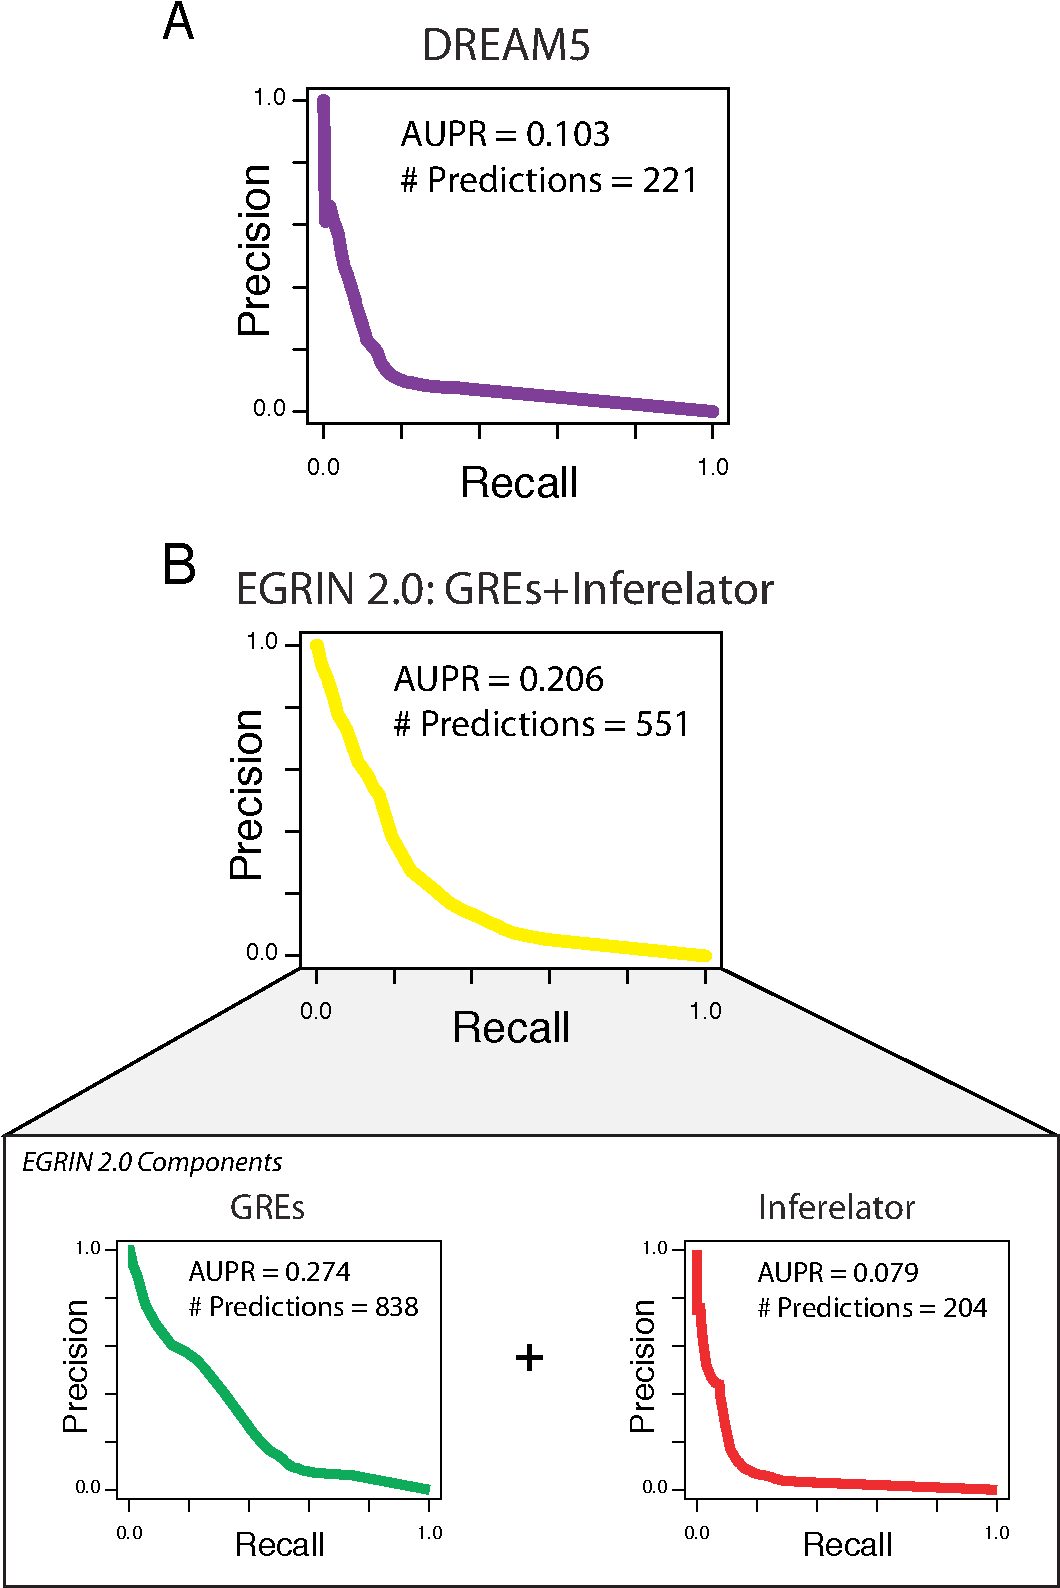
\includegraphics[width=0.8\linewidth]{figures/aupr.pdf}
\caption[Precision-recall performance for {\it E. coli}
  networks.]{\textbf{\DIFaddFL{Precision-recall performance for }\textit{\DIFaddFL{E. coli}}
    \DIFaddFL{networks.}} \DIFaddFL{Comparison of precision-recall performance on }{\it
    \DIFaddFL{E. coli}} \rdb\DIFaddFL{~gold-standard (Section
  \ref{section:eco:gold:standard}), for the DREAM5 ensemble network
  (A), compared to }\egrine \DIFaddFL{(B).  We compare the GRE-based and
  }\nwinf\DIFaddFL{-based networks (bottom)to the integrated }\egrine\DIFaddFL{~network
  (top). The integrated }\egrine\DIFaddFL{~network consists of an equal weighting
  of the GRE-based and }\nwinf\DIFaddFL{-based networks.  The }\egrine\DIFaddFL{~networks
  were inferred using the DREAM5 mRNA expression compendium (Section
  \ref{section:dream5_data_compendium}). Area under the curve (AUPR)
  and the number of true-positive predictions at a precision of 25\%
  are listed for each curve.}}
\label{fig:pr_curves}
\end{figure}

\DIFadd{Figure \ref{fig:argR_purR_networks} shows the inferred networks for
two genes regulated by PurR and ArgR (comparing predictions from
}\egrine\DIFadd{, }\tmsamp{CLR}\DIFadd{, DREAM5, and }\tmsamp{RegPrecise} \DIFadd{to the
annotations in }\rdb\DIFadd{). The result demonstrates that GRE-based
approaches can discover interactions that are not predicted using
direct approaches (See Section~\ref{section:gre_grn_construction}).
}

\begin{figure}[hp]
\centering
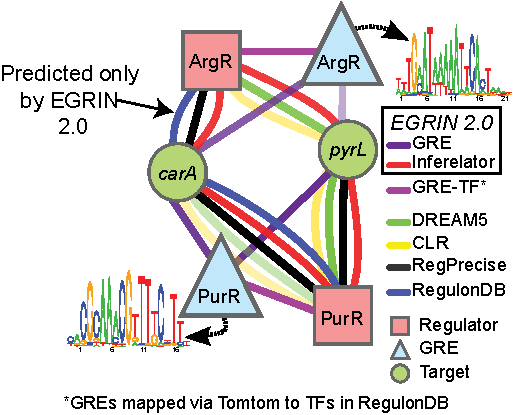
\includegraphics[width=0.75\linewidth]{figures/argR_purR_networks.pdf}
\caption[Integration of GRE discovery and Inferelator predictions
  yields comprehensive and detailed gene regulatory
  networks]{\textbf{\DIFaddFL{Integration of GRE discovery and Inferelator
    predictions yields comprehensive and detailed gene regulatory
    networks.}} \egrine\DIFaddFL{-inferred }\textit{\DIFaddFL{E. coli}} \DIFaddFL{regulatory subnetwork
  for two genes (green circles) in the PurR/ArgR regulon:
  }\textit{\DIFaddFL{carA}} \DIFaddFL{(}\textit{\DIFaddFL{b0032}}\DIFaddFL{) and }\textit{\DIFaddFL{pyrL}} \DIFaddFL{(}\textit{\DIFaddFL{b4246}}\DIFaddFL{).
  The }\egrine\DIFaddFL{~predictions are divided into GRE-based (dark violet) and
  Inferelator-based (red), and compared to predictions (or
  annotations) from other algorithms/databases (yellow: CLR; green:
  DREAM5 ensemble; black: RegPrecise; blue: RegulonDB). In two cases
  (ArgR$\rightarrow$carA and ArgR$\rightarrow$pyrL), }\egrine\DIFaddFL{~discovers
  regulatory interactions that were missed by either hand-curated
  databases or expression-based inference procedures.}}
\label{fig:argR_purR_networks}
\end{figure} 

\subsection{\DIFadd{Validation of condition-specific operon isoforms by tiling array transcriptome measurements}}

\DIFadd{We validated the prevalence of multiple, condition-specific
transcriptional isoforms from operons in }\eco\ \DIFadd{by measuring changes in
the transcriptome across growth, from lag-phase }\DIFaddend (\DIFdelbegin \DIFdel{Marbach et al., 2012). }\DIFdelend \DIFaddbegin \DIFadd{OD600 = 0.05) to late
stationary phase (OD600 = 7.3). The experimental platform and other
experimental details are described in Section
\ref{section:ecoarray}. We used multivariate recursive partitioning,
including signals from both relative changes in expression along the
growth curve, as well as raw RNA hybridization signal to call putative
transcription breaks as previously described \mbox{%DIFAUXCMD
\cite{Koide2009}
}%DIFAUXCMD
. To
determine the significance of our finding, we computed a $p$-value
describing the significance of the overlap between our predictions
(see Section \ref{section:condop}) and the experimental observations
using the cumulative hypergeometric distribution.
}\DIFaddend 

\DIFdelbegin \subsection{\DIFdel{Validation of conditional operons in tiling array transcriptome measurements}}
%DIFAUXCMD
\addtocounter{subsection}{-1}%DIFAUXCMD
\DIFdelend \DIFaddbegin \DIFadd{Figures \ref{fig:dpp_ecoli_expression}, \ref{fig:galE}, and
\ref{fig:ptsh} below depict several operons annotated with
condition-specific transcriptional isoforms. We have integrated GRE
elements discovered near break sites with the transcriptional
measurements.
}\DIFaddend 

\DIFdelbegin \subsection{\DIFdel{Global evaluation of fitness correlations}}
%DIFAUXCMD
\addtocounter{subsection}{-1}%DIFAUXCMD
%DIFDELCMD < 

%DIFDELCMD < %%%
\DIFdel{We defined gene modules using }\DIFdelend \DIFaddbegin \begin{figure}[hp]
\centering
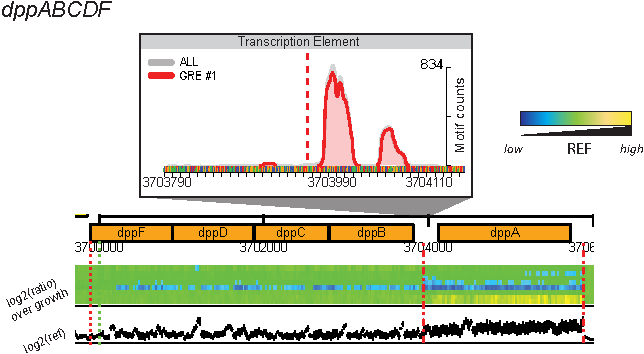
\includegraphics[width=0.8\linewidth]{figures/dpp_ecoli_expression.pdf}
\caption[GREs regulate multiple transcript isoforms from operons in
  {\it E. coli}, \textit{dppABCDF}]{\textbf{\DIFaddFL{GREs regulate multiple
    transcript isoforms from operons in }{\it \DIFaddFL{E. coli}}\DIFaddFL{,
    }\textit{\DIFaddFL{dppABCDF}}\DIFaddFL{.}} \DIFaddFL{GREs coincide with experimentally measured
  break sites. Three examples of experimentally determined
  transcription break sites (red dashed lines) in operons predicted by
  corems to be conditionally segmented. Expression levels of these
  regions were profiled across growth in rich media (heatmap). Inset
  contains region immediately surrounding a transcriptional break
  site, including counts of GREs discovered at these locations (as in
  Figure \ref{fig:nirH}).}}
\label{fig:dpp_ecoli_expression}
\end{figure}

\begin{figure}[hp]
\centering
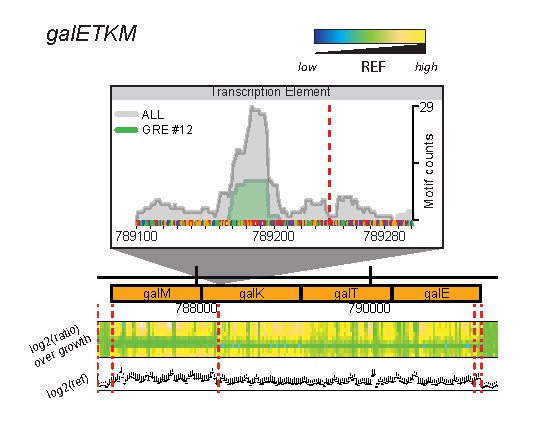
\includegraphics[width=0.8\linewidth]{figures/galE.pdf}
\caption[GREs regulate multiple transcript isoforms from operons in
  {\it E. coli}, \textit{galETKM}]{\textbf{\DIFaddFL{GREs regulate multiple
    transcript isoforms from operons in }{\it \DIFaddFL{E. coli}}\DIFaddFL{,
    }\textit{\DIFaddFL{galETKM}}\DIFaddFL{.}} \DIFaddFL{Caption details included in Figure
  \ref{fig:dpp_ecoli_expression}.}}
\label{fig:galE}
\end{figure}

\begin{figure}[hp]
\centering
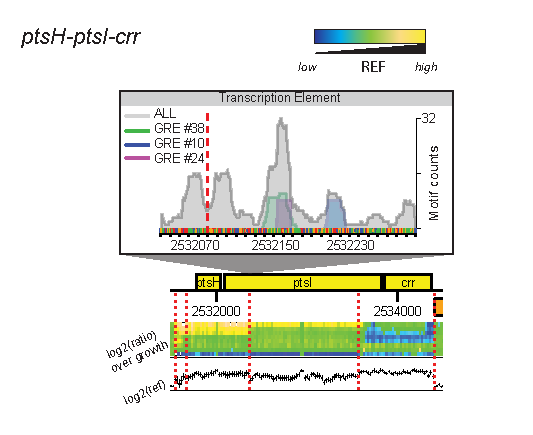
\includegraphics[width=0.8\linewidth]{figures/ptsh.pdf}
\caption[GREs regulate multiple transcript isoforms from operons in
  {\it E. coli}, \textit{ptsH-ptsI-crr}]{\textbf{\DIFaddFL{GREs regulate
    multiple transcript isoforms from operons in }{\it \DIFaddFL{E. coli}}\DIFaddFL{,
    }\textit{\DIFaddFL{ptsH-ptsI-crr}}\DIFaddFL{.}} \DIFaddFL{Caption details included in Figure
  \ref{fig:dpp_ecoli_expression}.}}
\label{fig:ptsh}
\end{figure}

\subsection{\DIFadd{Gene-gene co-fitness correlations in regulatory modules}}

\DIFadd{To assess the phenotypic consequences of co-regulation in corems, we
assessed whether genes grouped into corems had significantly similar
fitness consequences in many environments (}\ie\DIFadd{, the effect of deleting
one gene is highly similar to the effect of deleting the other across
many environments). We used the high-throughput fitness screen
described in Section \ref{section:fitness} to quantify these
relationships.
}

\DIFadd{We compared the enrichment for high co-fitness relationships in corems
to other ways of assigning co-regulatory modules, including regulons
(RegPrecise, RegulonDB), operons, and WGCNA. The gene modules for
}\DIFaddend regulons (annotated in \DIFdelbegin \DIFdel{RegulonDB or RegPrecise) by grouping together genes that were annotated as
controlled by }\DIFdelend \DIFaddbegin \rdb\DIFadd{~or }\tmsamp{RegPrecise}
\DIFadd{\mbox{%DIFAUXCMD
\cite{Novichkov2013}
}%DIFAUXCMD
) consisted of genes annotated to }\DIFaddend a common TF. \DIFdelbegin \DIFdel{Using }\DIFdelend \DIFaddbegin \DIFadd{For
WGCNA, we assigned modules using }\DIFaddend the same community detection
procedures that we used to define corems from the \DIFdelbegin \DIFdel{EGRIN 2.0 ensemble
,
we computed }\DIFdelend \DIFaddbegin \egrine\DIFadd{~ensemble
(See \ref{section:gBg}). The }\DIFaddend gene co-expression modules \DIFaddbegin \DIFadd{were computed
}\DIFaddend from the weighted \DIFdelbegin \DIFdel{WGCNA
}\DIFdelend \DIFaddbegin \tmsamp{WGCNA} \DIFaddend adjacency matrix.
\DIFdelbegin \DIFdel{We }\DIFdelend \DIFaddbegin 

\DIFadd{For the results presented in Figure~2B, we }\DIFaddend compared the distributions
of Pearson correlations between relative changes in fitness across
pairs of genes within each module, using the one-tailed
Kolmogorov-Smirnov test (KS-test). \DIFaddbegin \DIFadd{We report the KS $D$-statistic. }\DIFaddend The
precision/recall characteristics for each model are contained in Table\DIFaddbegin \DIFadd{~}\DIFaddend E5.
\DIFaddbegin 

\DIFadd{We extended this analysis by investigating whether the enriched high
co-fitness gene-gene relationships in corems consist of relationships
that could be described fully by regulons or operons. To answer this
question, we removed all gene pairs from corems that are also present
in operons or regulons and computed the KS-test again (Figure
\ref{fig:fitness_wo_operons}). We still observe a significant number
of high co-fitness relationships, suggesting that corems capture
physiologically meaningful co-regulatory relationships between genes
that cannot be explained by existing paradigms.
}

\begin{figure}[hp]
\centering
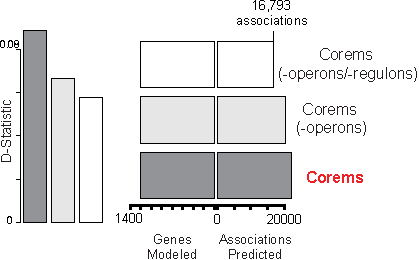
\includegraphics[width=0.75\linewidth]{figures/fitness_wo_operons.pdf}
\caption[\egrine~models highly correlated co-fitness relationships
  that cannot be explained by operons or
  regulons]{\textbf{\egrine\DIFaddFL{~models highly correlated co-fitness
    relationships that cannot be explained by operons or regulons.}}
  \DIFaddFL{(Left) Enrichment for highly correlated, pairwise fitness
  measurements in gene knock outs across 324 conditions before and
  after removing gene associations annotated by operons
  (MicrobesOnline) and regulons (RegulonDB and RegPrecise)
  (KS-test,$D$-statistic). Two-thirds of gene-pairs with most highly
  correlatedfitness within corems are not annotated by operons or
  regulons. (Right) Number of genes and associations predicted.}}
\label{fig:fitness_wo_operons}
\end{figure}
 \DIFaddend